\documentclass[12pt]{article}
\usepackage[utf8]{inputenc}
\usepackage[T1]{fontenc}
\usepackage{graphicx}
\usepackage{xcolor}

%%novalidate

\usepackage{tikz}
\usepackage{calc}
\usepackage{booktabs}


% colors
\definecolor{color1}{HTML}{000060}
%\definecolor{color1}{HTML}{8C260F}
\definecolor{color2}{HTML}{333333}


% fonts
\usepackage{lmodern}
\renewcommand{\sfdefault}{lmss}
\renewcommand\familydefault{\sfdefault}
%%%


\usepackage{geometry}
\geometry{a4paper,
hmargin=20mm,vmargin=20mm,
head=0ex,foot=3ex}

\linespread{1.3}

\usepackage[hang]{caption}
\DeclareCaptionFormat{upper}{#1#2\uppercase{#3}\par}
\captionsetup{labelfont={bf,color=color2},textfont={normalsize,color=color2},format = upper,figurename=FIGURE,tablename=TABLE}

%%% fancy sections
\usepackage{titlesec}
%\titleformat{\chapter}{\sffamily\LARGE\bfseries\scshape\color{color1}}{\thechapter}{1em}{}[\titlerule]
\titleformat{\section}{\color{color1}\sffamily\Large\bfseries\uppercase}{\thesection}{1em}{}[\titlerule]
\titleformat{\subsection}{\color{color1}\sffamily\large\bfseries\uppercase}{\thesubsection}{1em}{}
\titleformat{\subsubsection}{\color{color1}\sffamily\bfseries\uppercase}{\thesubsubsection}{1em}{}
%%%

% head and foot
\usepackage{fancyhdr}
\pagestyle{fancy}
\lhead{}
\chead{}
\makeatletter
\rhead{\color{color2}\@date}
\makeatother
\newlength{\myheight}
\lfoot{
\settoheight{\myheight}{\thepage}
\raisebox{-2ex-0.5\myheight}{
\includegraphics[height=4ex]{images/logo}}
}
\cfoot{\color{color2}Cupboard: Requirements Specfication}
\rfoot{\color{color2}\thepage}
\renewcommand\headrulewidth{0pt}
\renewcommand\footrulewidth{0pt}

% custom titlepage
\makeatletter
\newcommand*\DefVar[1]{\@namedef{#1}##1{\global\@namedef{get#1}{##1}}}
\DefVar{summary}
\renewcommand{\maketitle}{
\begin{center}

\begin{tikzpicture}
    \node[draw=none,%color1,line width=0.4pt,
      fill=color1,
      inner sep = 10pt,
      text width=\textwidth-20pt,
      text centered
    ] {\color{white}\sffamily\bfseries\huge\@title};
\end{tikzpicture}
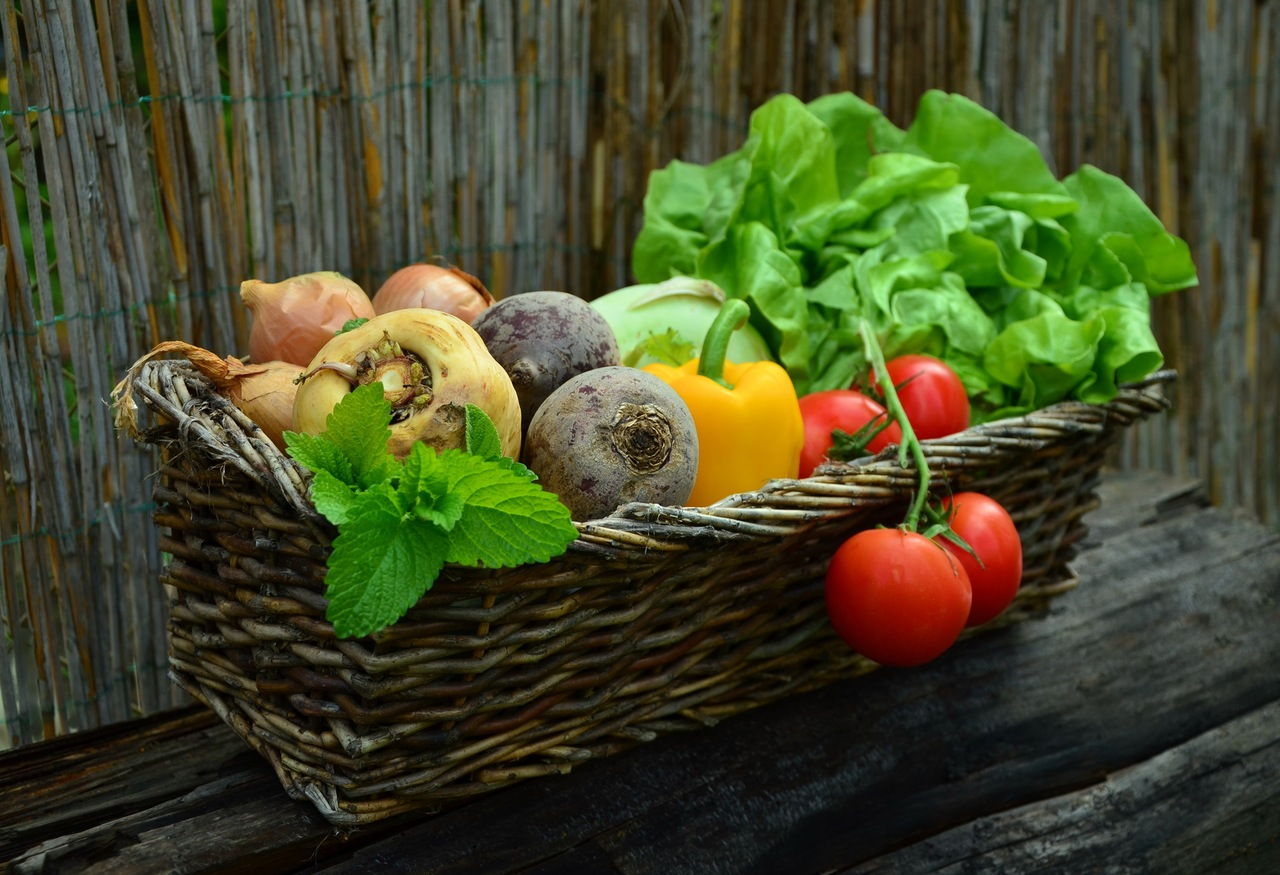
\includegraphics[width=\textwidth]{images/opening}\par
\sffamily\bfseries\Large\@author\par
\bigskip\medskip
{\color{color2}\normalfont\normalsize\textbf{Summary:}\\
\getsummary}
\end{center}
\clearpage
}
\makeatother
%%%

%%% fancy boxes
\usepackage{tcolorbox}
\usepackage{wrapfig}
\def\fullboxbegin{
\bigskip
\begin{tcolorbox}[colback=color1,colframe=color1,coltext=white,arc=0mm,boxrule=0pt]
}
\def\fullboxend{\end{tcolorbox}\medskip}
%
\def\leftboxbegin{
\begin{wrapfigure}{l}{0.5\textwidth}
\begin{tcolorbox}[colback=color1,colframe=color1,coltext=white,arc=0mm,boxrule=0pt]
}
\def\leftboxend{
\end{tcolorbox}
\end{wrapfigure}
}
%
\def\rightboxbegin{
\begin{wrapfigure}{r}{0.5\textwidth}
\begin{tcolorbox}[colback=color1,colframe=color1,coltext=white,arc=0mm,boxrule=0pt]
}
\def\rightboxend{
\end{tcolorbox}
\end{wrapfigure}
}
%
\newcounter{frames}
\def\frameboxbegin#1{
\bigskip
\refstepcounter{frames}
\begin{tcolorbox}[colback=white,colframe=color1,arc=0mm,title={\MakeUppercase{\textbf{Frame \arabic{frames}}: #1}}]
}
\def\frameboxend{
\end{tcolorbox}
}
%%%

%custom Requirements titles
\usepackage{titlesec}
%\usepackage{hyperref}
%Funtional
\titleclass{\requirement}{straight}[\subsubsection]
\newcounter{requirement}
\titleformat{\requirement}
  {\color{color1}\sffamily\bfseries}{}{0em}
  {\refstepcounter{requirement}FR \therequirement:~}
\titlespacing*{\requirement}{0pt}{3.25ex plus 1ex minus .2ex}{1.5ex plus .2ex}

\setcounter{tocdepth}{4}
\makeatletter
  \def\toclevel@requirement{5}
  \def\l@requirement{\@dottedtocline{5}{3.8em}{3.2em}}
\makeatother
%%%


%requirements table enviromnent
\newenvironment{reqtable}
{
    \medskip
    \begin{tabular}{|p{3.5cm}|p{11cm}|}
    \hline
}
{\end{tabular}}


\usepackage{lipsum}

%%%%%%%%%%%%%%%
% Title Page
\title{Cupboard:\\Requirements Specfication}
\author{Team 8:\\Clare Doran, Abdul Ghani, Ucizi Mafeni, Luke Needham, Soumya Singh}
\date{\today}
\summary{
A web app built with the intention of helping reduce food waste
}
%%%%%%%%%%%%%%%

\begin{document}
\maketitle

\tableofcontents
\clearpage

\section{Introduction}
7 million tonnes of food goes to waste in the UK, more than half of which is 
edible (https://www.lovefoodhatewaste.com/node/2472).
Meanwhile,  many people throughout the country struggle to put together enough 
money for food, with food banks becoming busier every year
(https://www.trusselltrust.org/2015/11/18/uk-foodbank-use-still-at-record-levels-as-hunger-remains-major-concern-for-low-income-families/)

Cupboard aims to be a system that allows users to painlessly find and share food
that would otherwise go to waste. It should be quick and easy to use as it is
too easy to just throw away food. 
It will also allow users to arrange collection in a manner that does not force
them to disclose their house address or any other details they wish to keep
private.


\section{Project Scope}
Cupboard will facilitate the sharing of food between users. It will do so in a
manner that is as simple as possible, as we want to discourage people from
taking the easy route of simply binning food they wont eat.
There will be a simple points-based system and a ranking system in order to
encourage sharing of food and reassure other users that the quality of food is
likely to be good. When some food has been ‘successfully exchanged’ both
parties will get points and will be able to rate each other. If users wish to
participate, there will be a simple public leaderboard.
Users can set their dietary requirements (allergies, religious etc.) and have
results automatically filtered. 
There will be a messaging system (in order to arrange collection) and a comments
system (in order to view interest in the item and ask questions).


\section{Domain Analysis}
There are a couple of examples of food sharing sites/apps such as:
\begin{itemize}
    \item foodsharing.de(https://foodsharing.de/): A German food sharing site
        that allows users (just like our site) to trade food that is going out
        of date with other users to reduce food waste.
        However it is only available in Germany.
    \item Olio (https://olioex.com/): Mobile app with strong UK presence.
        A key distinguishing feature is "Drop Boxes".
        These are local stores/cafes where users can drop off food they'd like
        to be shared.
    \item SharingFood
        (https://itunes.apple.com/us/app/sharing-food/id992111062?mt=8):
        Mobile app based in Italy.
        Seems to be fairly new and so has a very small user base.
\end{itemize}


\section{Proposed Deliverables}
(Gantt Chart Goes here)

\section{Identified, Risks, Assumptions, Dependencies and Constraints}
\begin{itemize}
    \item User Location: How much information about the user's location can we
        make publicly available without putting their security ar risk?
    \item Assuming google maps should be able to find the addresses entered by
        the user.The location functionality is completely dependent on the
        Google Maps API.
\end{itemize}

\section{Solution Requirements}
\subsection{Functional Requirements}
\requirement{User sign up}
Users can sign up via email and eventually via social media. As a minimum, they
will first enter a username, email and password – then be taken to a page where
they can optionally set a profile picture, location, and any dietary
requirements.

\requirement{User sign up}
Users will be able to list an item of food. The minimum amount of information
will be a title. Optionally, they may add a picture, location, description,
expiry date, and set the dietary requirement flags. If the user has set their
location, it will be automatically added.

\requirement{Messaging, comments, and collection of food}
Messaging (private communication, to exchange exact addresses etc.) and
comments (questions that others may be interested in, expressing interest)
will be implemented.
After food is collected, both parties will have their
scores and ratings affected appropriately and the item will be moved to a
separate ‘history’ database.
(Items can also be deleted, and not moved to a users history).

\requirement{Search}
Searching will be implemented in a dynamic fashion using AJAX. By default,
items will be listed by location.

\requirement{Points and ratings}
A simple points/ratings system will be implemented. When some food has been
shared, the donor receives three points and the collector gets a single point.
Each party can then rate their experience with the other out of 5.
If the user wishes, they may be displayed on a public leaderboard.


\subsection{Non-Functional Requirements}
\begin{itemize}
    \item Items will be stored in only one location and so will be consistent.
    \item Animations and transitions will be simple and fluent in order to keep
        the interface responsive.
    \item All functionalities will be supported on all devices, apart from
        wearables.
\end{itemize}


\section{Development Approach}

\subsection{Key Summary}
We've decided to use PHPStorm as the main IDE. Ultimately we hope to host the
Database (and possibly website) on AWS. We will mainly collaborate using
Github and Slack (and occasionally email).

Though we'll all inevitably contribute to both sides of the site, we've
decided to split the work as follows:
\begin{itemize}
    \item \textbf{Design and Frontend:} Clare, Ucizi and Luke
    \item \textbf{Database and Backend:} Soumya and Abdul
\end{itemize}

\subsection{Development Stack}
\begin{itemize}
    \item PHP (Database and other backend features)
    \item HTML/CSS
    \item SQL
    \item Javascript (Client-side features)
    \item Bootstrap (Simplifies mobile compatibility)
    \item Git
\end{itemize}


\section{References}
\end{document}
